\documentclass[aspectratio=169]{beamer}
\usepackage{lmodern}
%\usetheme{Madrid}
%\usecolortheme{giantoak}
\newcommand*\oldmacro{}
\let\oldmacro\insertshorttitle
\renewcommand*\insertshorttitle{\oldmacro\hfill\insertframenumber\,/\,\inserttotalframenumber}
\usepackage[framemethod=tikz]{mdframed}

%\usepackage{beamerthemesplit}
\usepackage{textpos}
\usepackage{pgf}
\usepackage{ulem}
%\logo{\pgfputat{\pgfxy(0,-.4)}{\pgfbox[right,base]{\includegraphics[height=1.0cm]{logo.jpg}}}}
%\newcommand{\nologo}{\setbeamertemplate{logo}{}}
\usepackage{booktabs}
\usepackage{graphicx}
\theoremstyle{principle}
\newtheorem*{principle}{Design Principle}


\titlegraphic{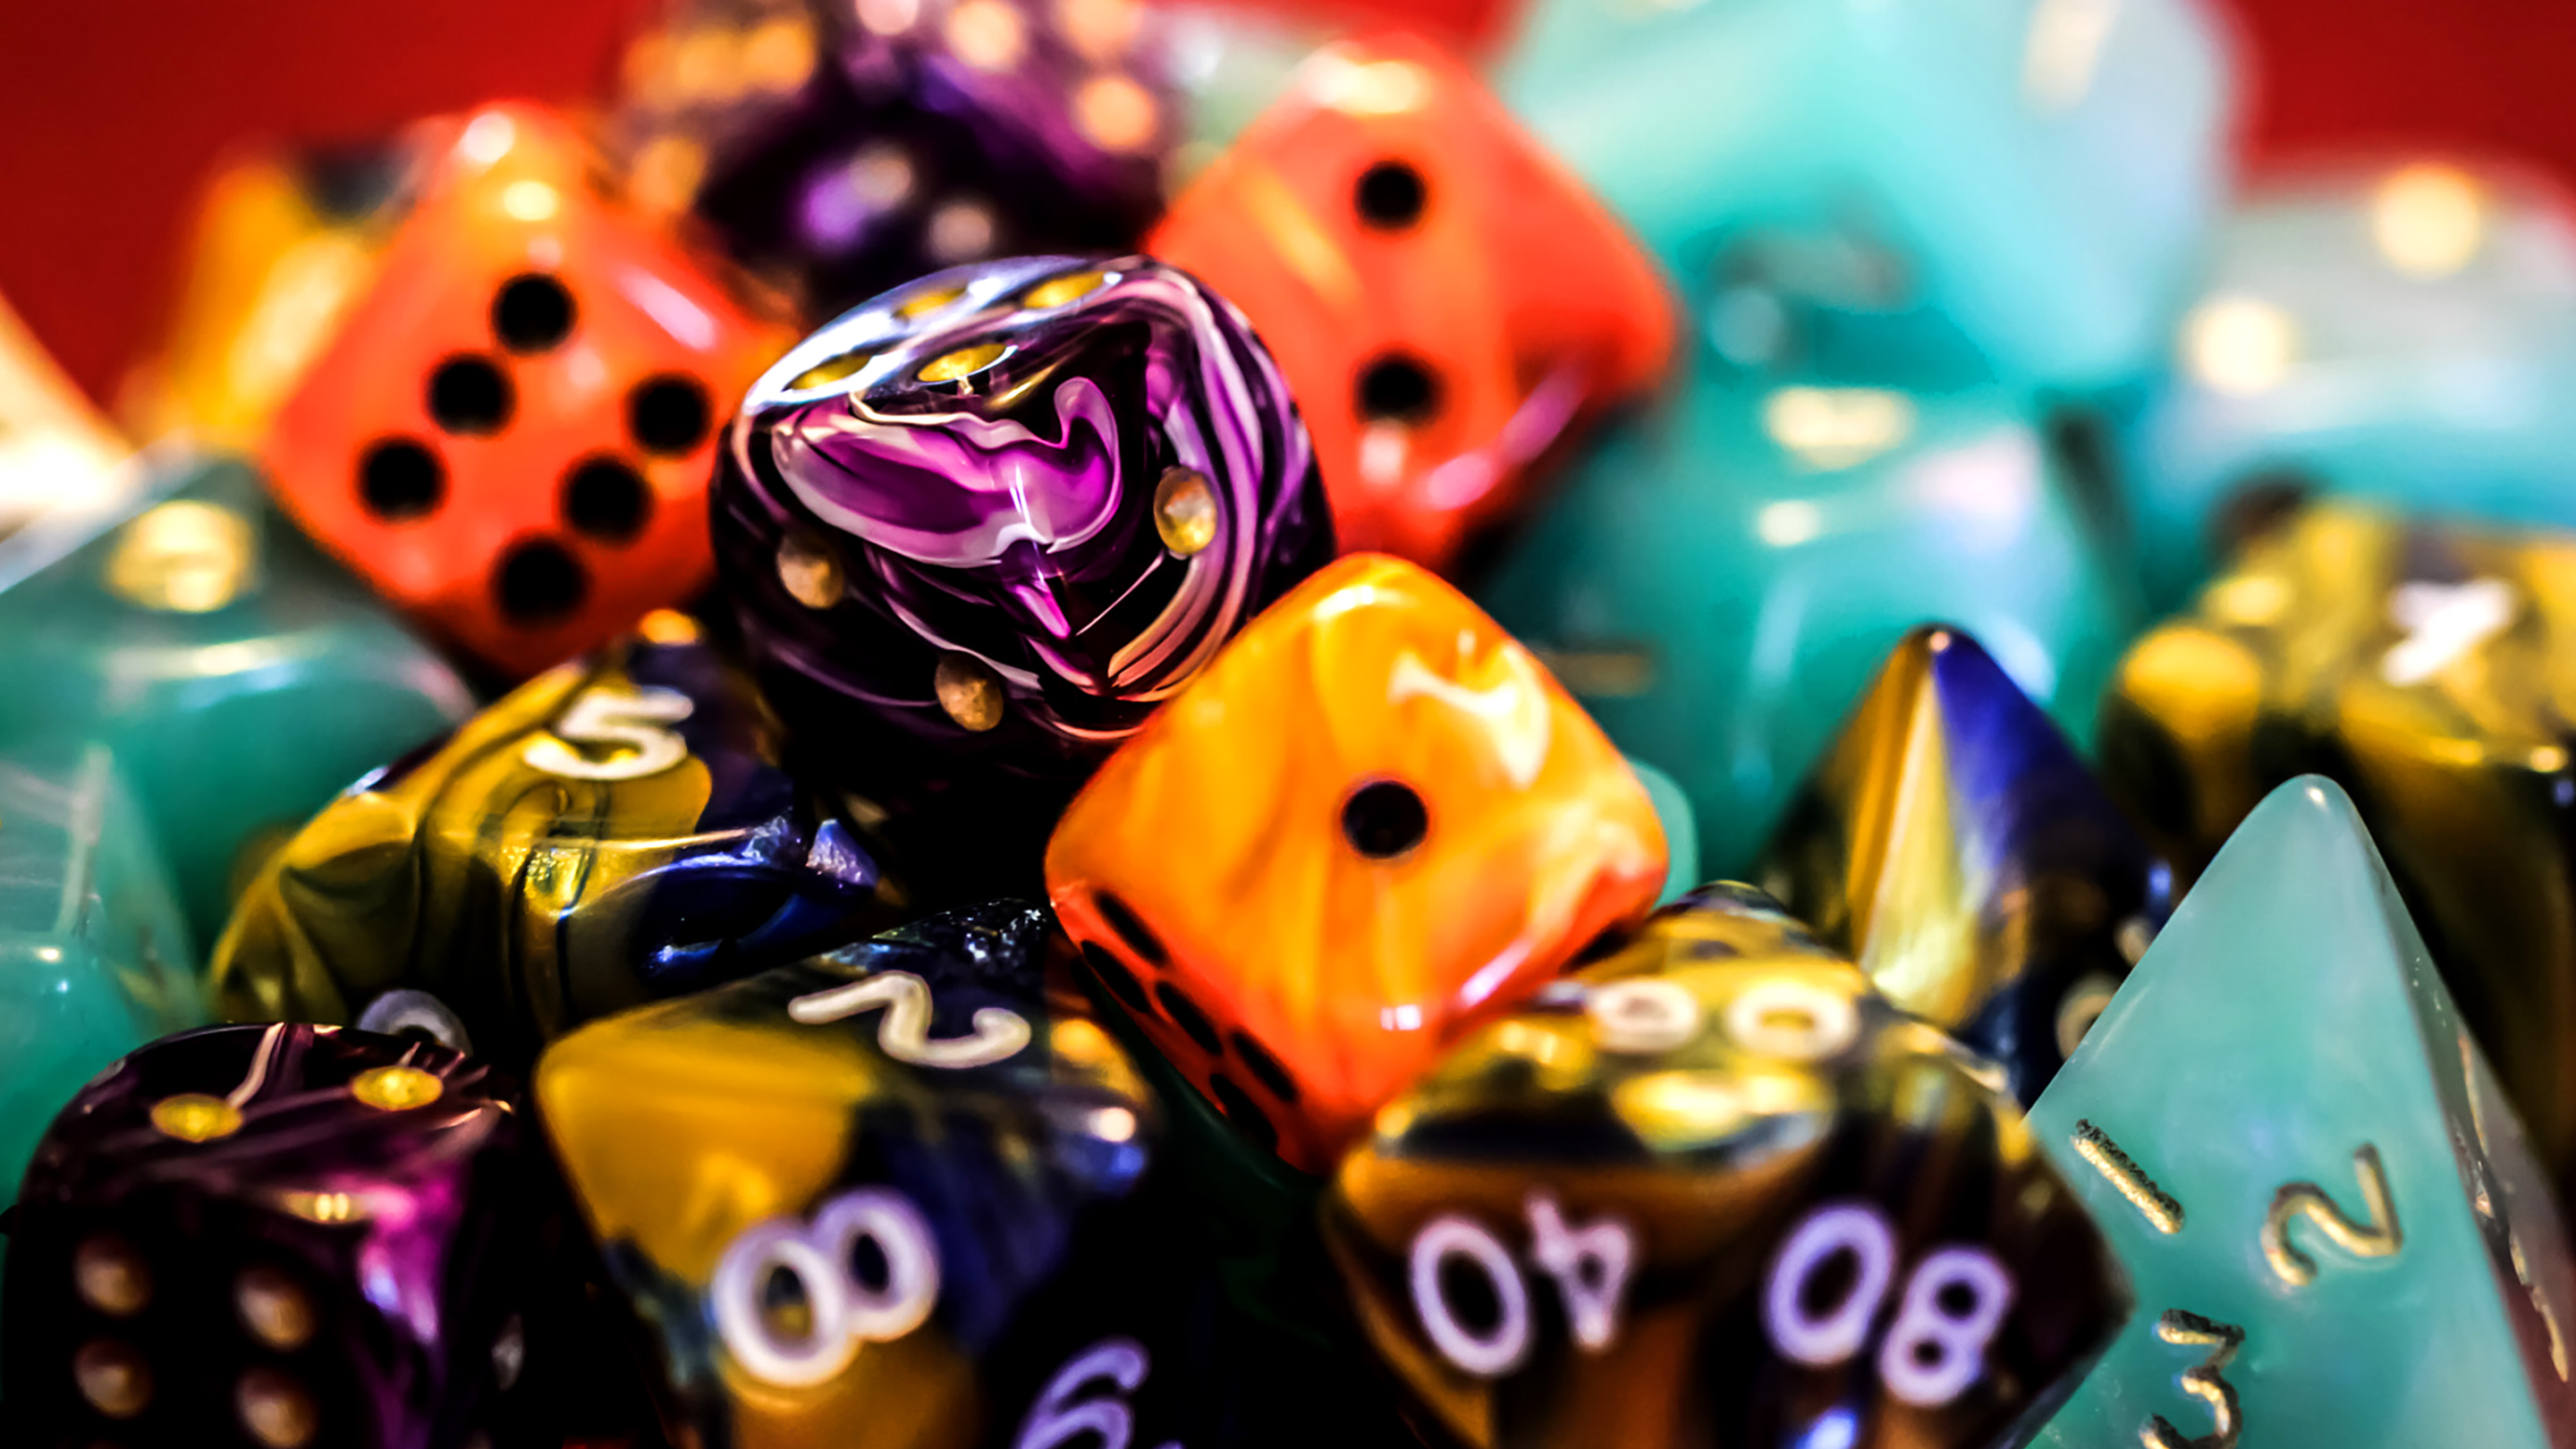
\includegraphics[width=1.0\paperwidth]{dice.jpg}}

\title{Amendments}
%\author[Jeremy Kedziora]{Wind Data Science Team\\
%\small{Uptake}}
\date{}

\begin{document}

%{
%%\nologo
%\begin{frame}
%    \maketitle
%\end{frame}
%}
%pages 1-7, 8-9, 14-15.


{
%  \usebackgroundtemplate{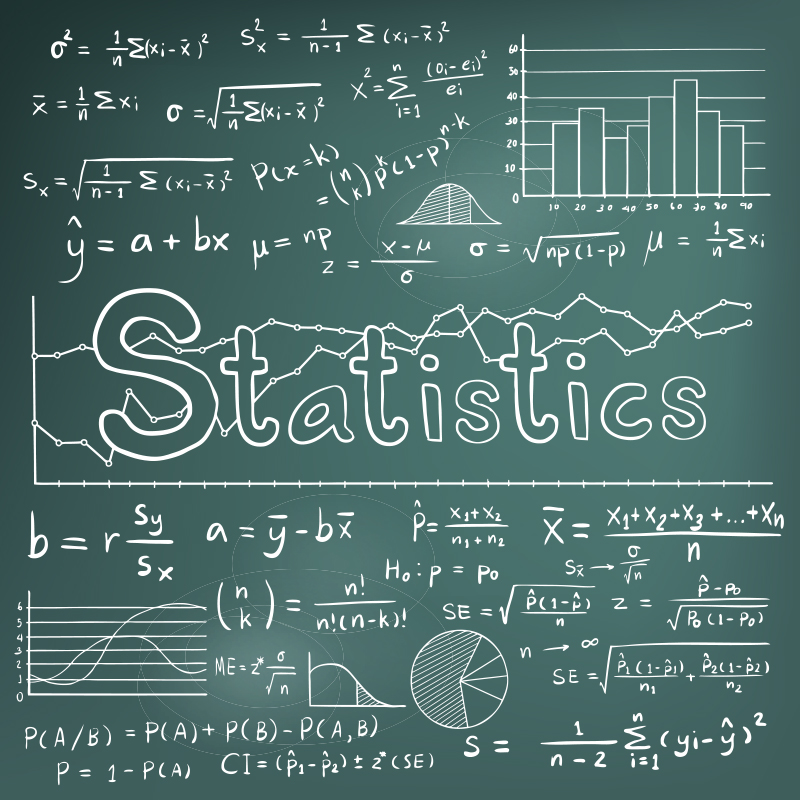
\includegraphics[width=1.0\paperwidth]{statistics-review.jpg}}
  \usebackgroundtemplate{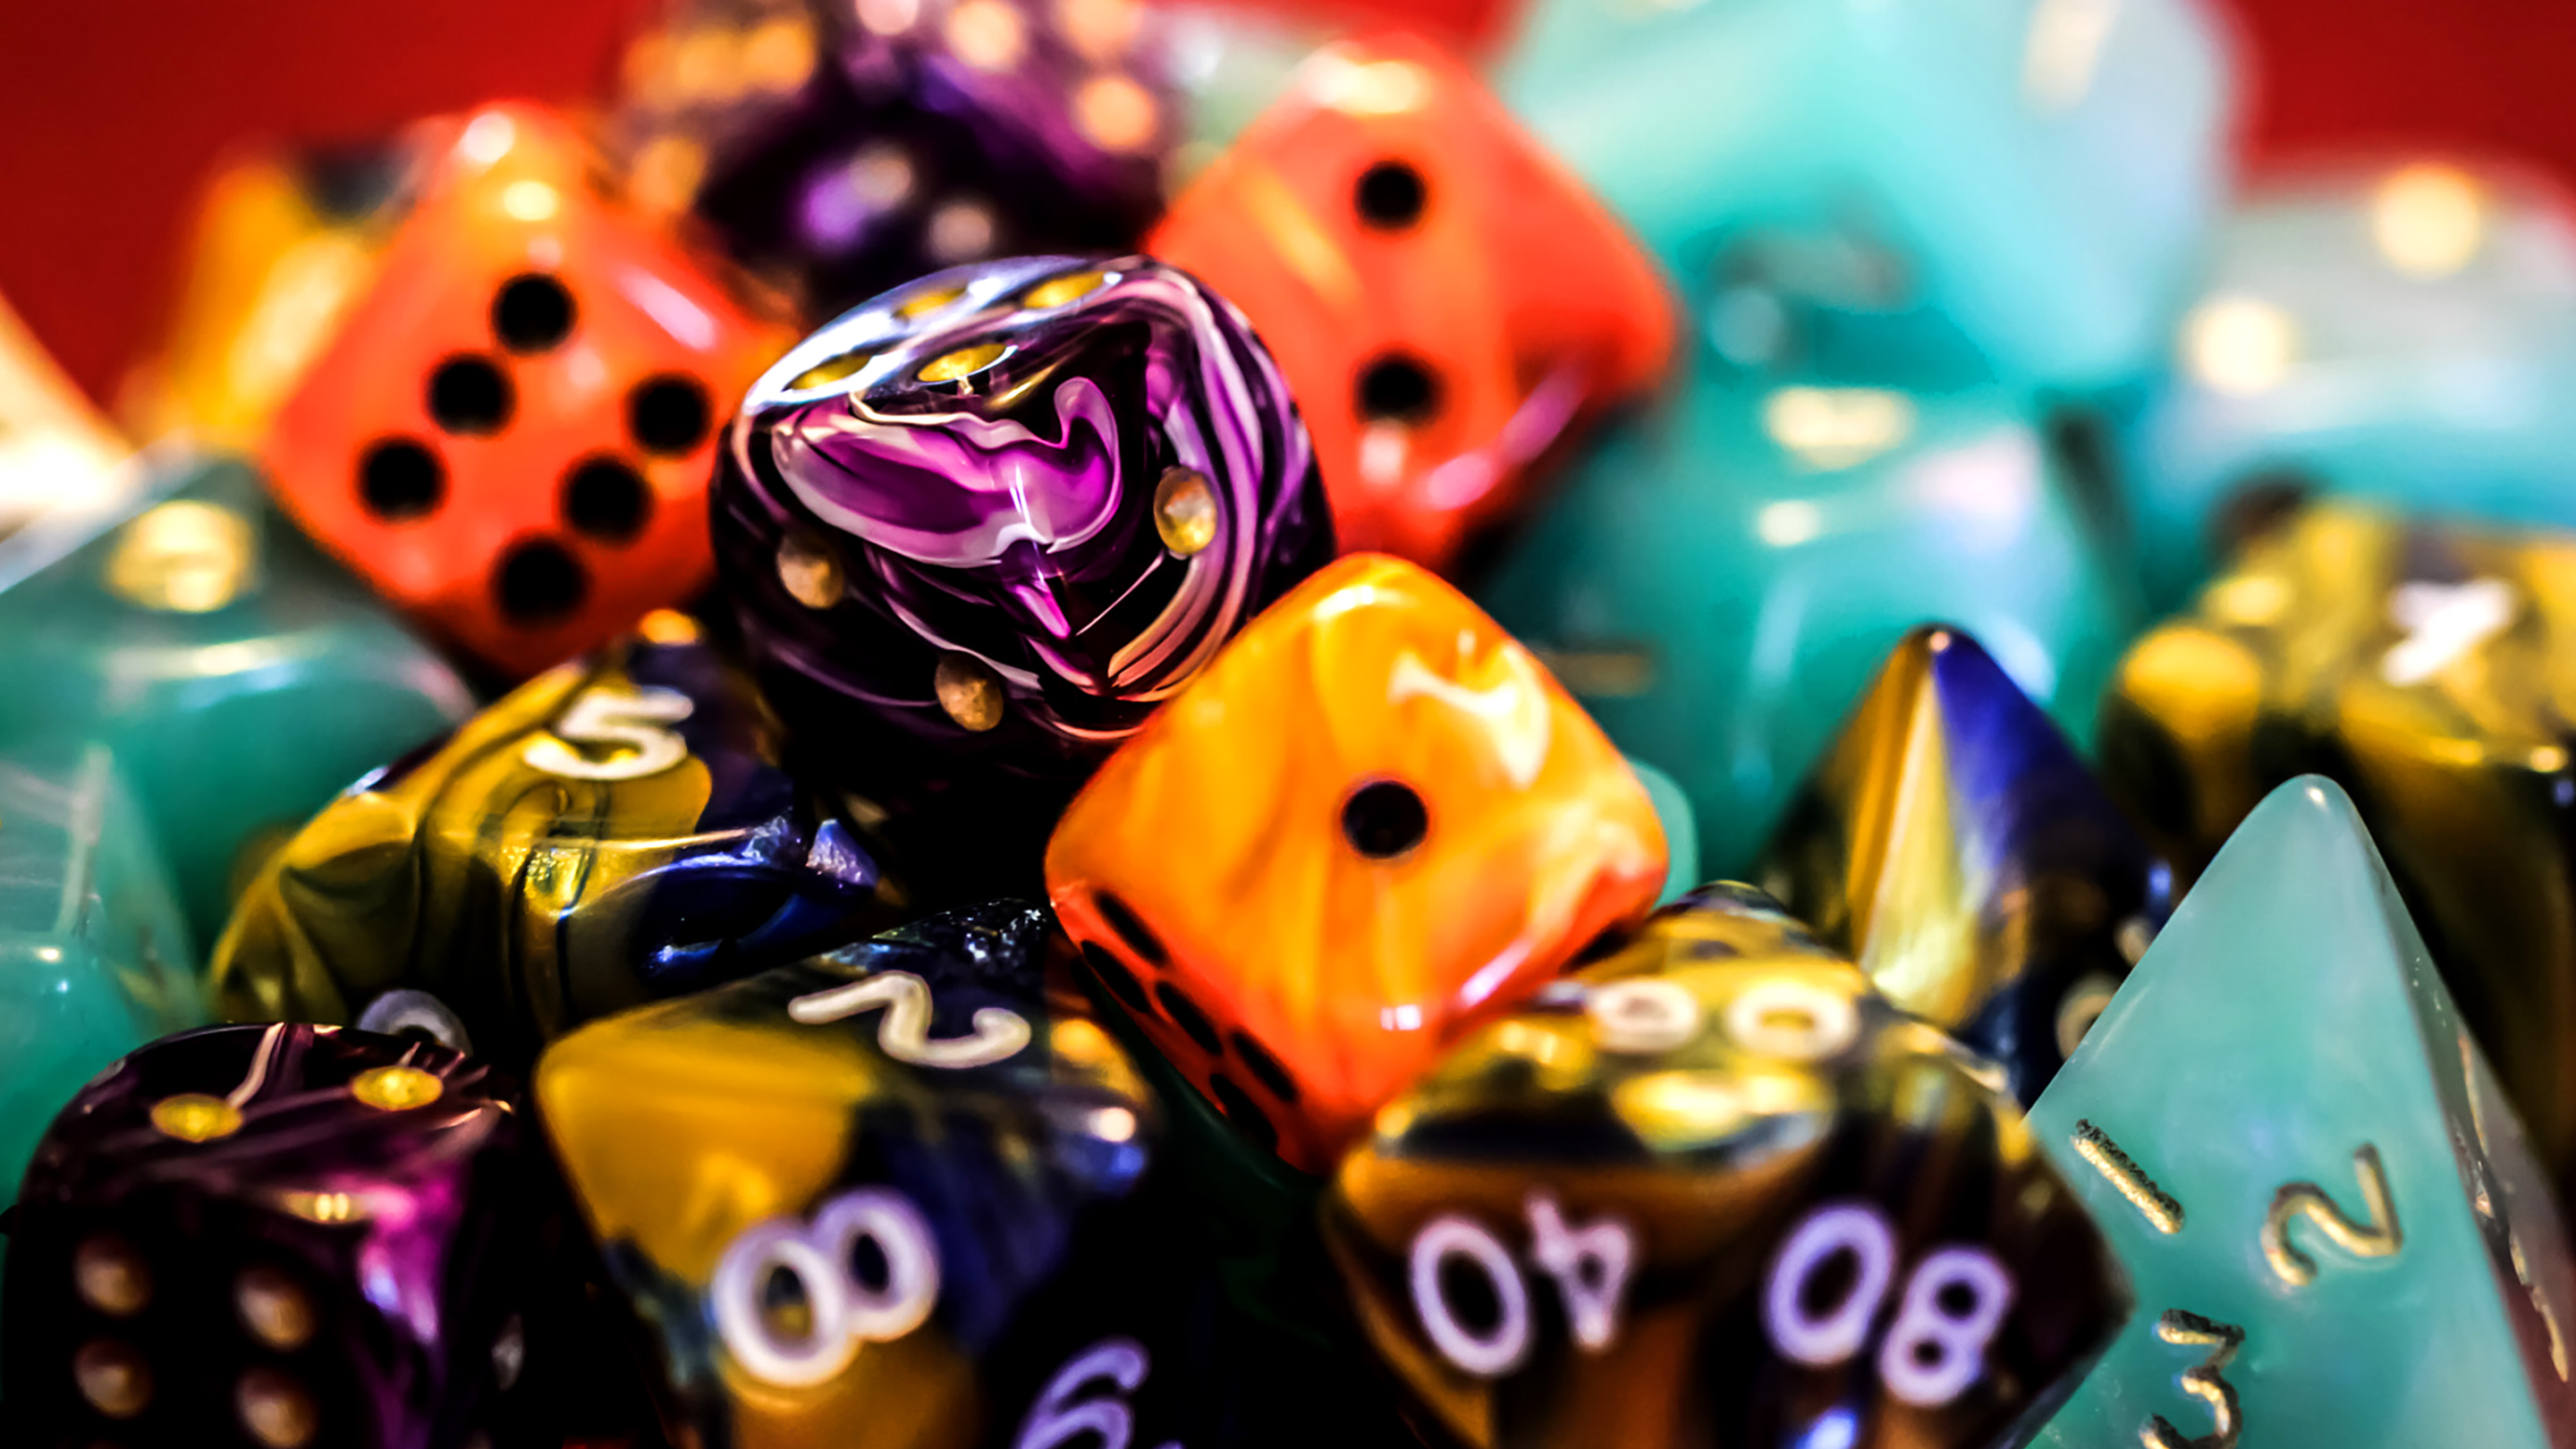
\includegraphics[scale=0.2]{dice.jpg}}
  \begin{frame}[plain]
  
\begin{mdframed}[tikzsetting={draw=white,fill=white,fill opacity=0.6,draw opacity=0.4,
               line width=0pt},backgroundcolor=none,leftmargin=20,
               rightmargin=20,innertopmargin=4pt]
\begin{center}
\Huge \textbf{Random Variables and Probability}
\end{center}
\end{mdframed}

  \end{frame}
}

%most reliant on human cognition
%limited only by cognition
%hypothesis generating scheme often functioning as a gateway into more statistical analysis

%%@@@@@@@@@@@@@@@@@@@@@@@@@@@@@@@@@@@@@@@@@@@@@@@@@
%\begin{frame}
%\frametitle{Napoleon's Progress}
%\begin{center}
%
\includegraphics[scale=0.4]{experiment.png}
%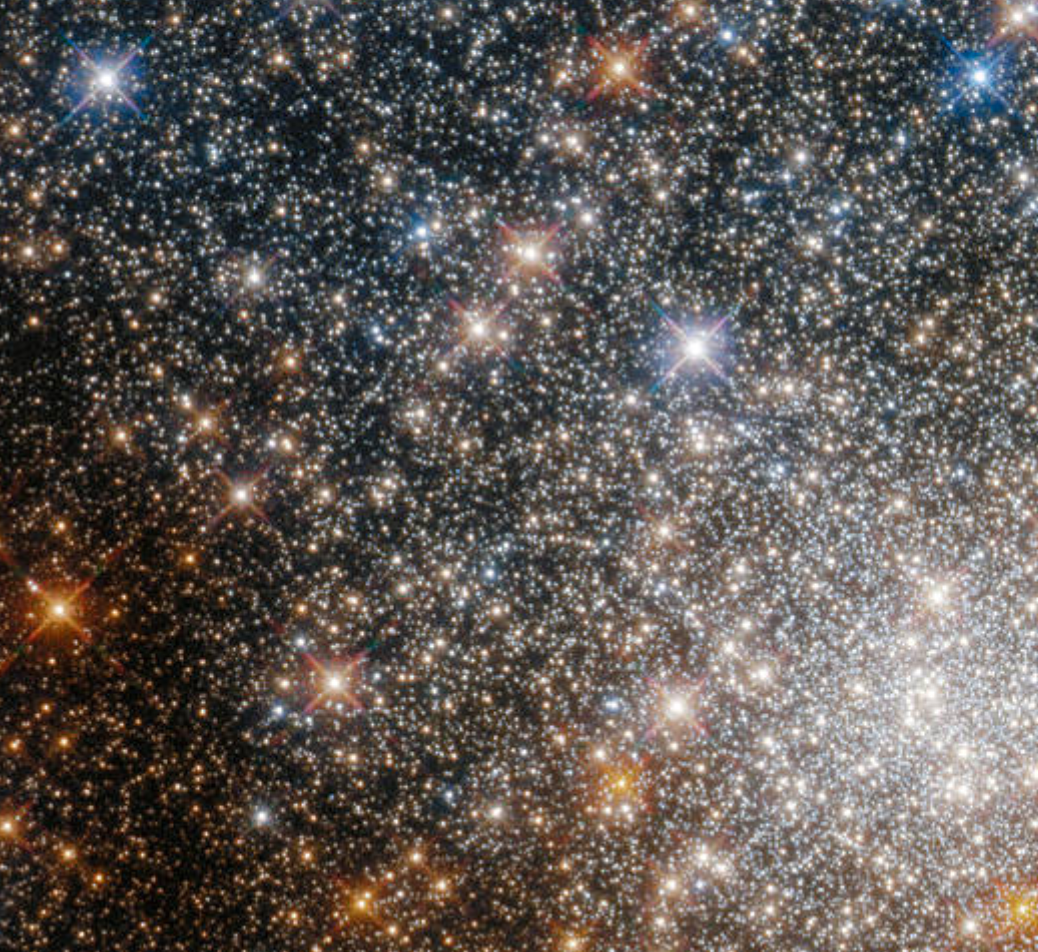
\includegraphics[scale=0.35]{stars.png}
%\end{center}
%
%\end{frame}

%@@@@@@@@@@@@@@@@@@@@@@@@@@@@@@@@@@@@@@@@@@@@@@@@@
\begin{frame}
\frametitle{Today:}

\begin{itemize}
\item Talk about a little bit of math;
\bigskip
\bigskip
\bigskip

\item Introduce the ideas of random variables and probability;
\bigskip
\bigskip
\bigskip

\item Discuss Bernoulli, Binomial, and Normal random variables;
\bigskip
\bigskip
\bigskip

\item Compute these distributions in R.

\end{itemize}

\end{frame}

%@@@@@@@@@@@@@@@@@@@@@@@@@@@@@@@@@@@@@@@@@@@@@@@@@
\begin{frame}
\frametitle{Motivation -- reasoning about voters...}

\begin{columns}
\begin{column}{0.5\textwidth}

\begin{itemize}
\item Cavalier Johnson: a political candidate running a campaign for Mayor of Milwaukee;
\bigskip

\item Johnson's campaign claims that he will win the election -- in this case that means getting more than 50\% of votes from Milwaukee voters;
\bigskip

\item How to assess the Johnson campaign claim?  Conduct an experiment:
\begin{itemize}
\item \textbf{Sample} $n$ voters from Milwaukee;
\item Record the number of voters who will vote for Johnson.
\end{itemize}

\end{itemize}

\end{column}
\begin{column}{0.5\textwidth}
\begin{center}
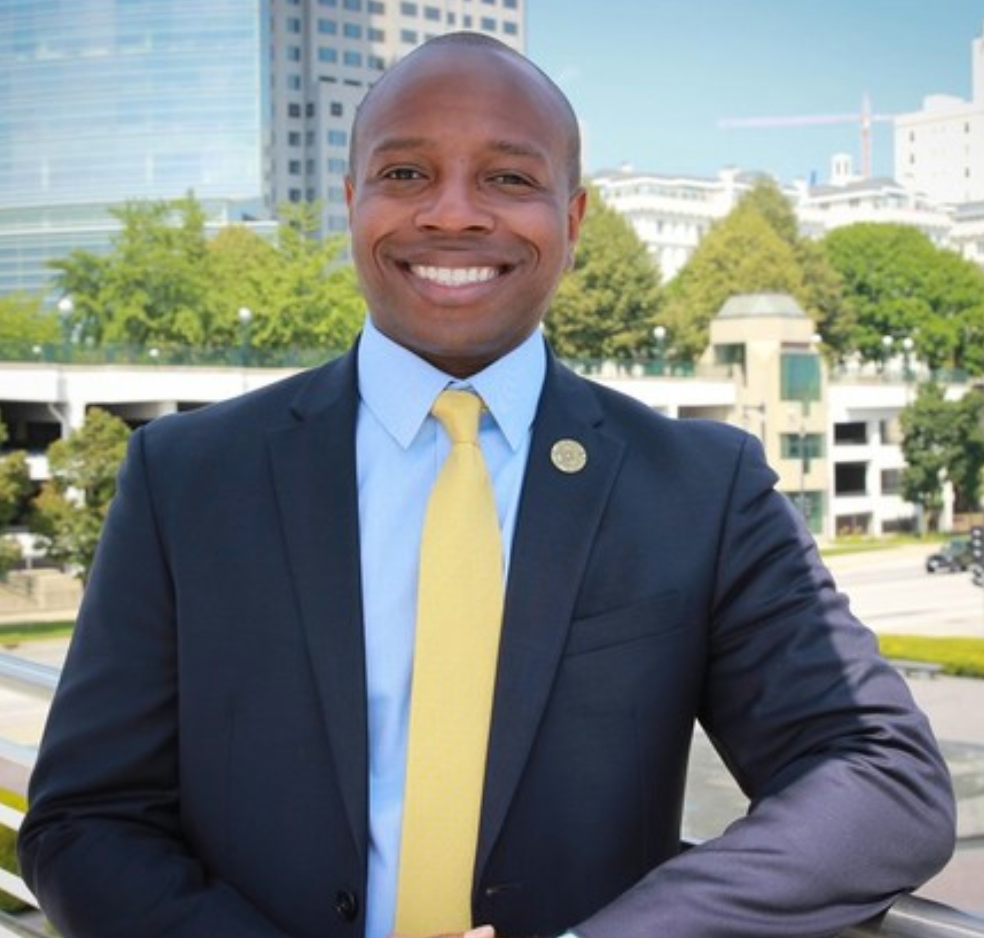
\includegraphics[scale=0.4]{Johnson.png}
\end{center}
\end{column}
\end{columns}

\end{frame}

%@@@@@@@@@@@@@@@@@@@@@@@@@@@@@@@@@@@@@@@@@@@@@@@@@
\begin{frame}
\frametitle{A little bit of math...}

\begin{itemize}
\item \textbf{Sum} -- shorthand to write adding up a bunch of stuff:
\begin{align*}
\sum_{i=1}^{5}x_i = x_1 + x_2 + x_3 + x_4 + x_5;
\end{align*}

\item[]\color{white} \textbf{Function} -- a relationship between variables with a \textbf{dependent variable} that depends on an \textbf{independent variable(s)};
\begin{itemize}
\item[]\color{white} We write the dependent variable as $f$, $y$, or $p$ (but not always!), the independent variable as $x$, and the relationship between them as $f(x)$;
\item[]\color{white} Example: $f(x) = 2x + 3$;
\item[]\color{white} Example: $f(x,z) = 2x + 3z$;
\item[]\color{white} Example: $y(x_1,x_2,\beta_0,\beta_1,\beta_2) = \beta_0 +\beta_1x_1 + \beta_2x_2$;
\item[]\color{white} Example -- from our classes on causal inference: $Y_i(T)$;
\item[]\color{white} Example -- from our classes on causal inference: $Y_i(T,C,C,T,C,T,C)$;
\end{itemize}
\bigskip

\item[]\color{white} \textbf{Exponentiation} -- we write $\mbox{exp}\{x\}$ and this is shorthand for $2.718^x$;

\end{itemize}

\end{frame}

%@@@@@@@@@@@@@@@@@@@@@@@@@@@@@@@@@@@@@@@@@@@@@@@@@
\begin{frame}
\frametitle{A little bit of math...}

\begin{itemize}
\item \textbf{Sum} -- shorthand to write adding up a bunch of stuff:
\begin{align*}
\sum_{i=1}^{5}x_i = x_1 + x_2 + x_3 + x_4 + x_5;
\end{align*}

\item \textbf{Function} -- a relationship between variables with a \textbf{dependent variable} that depends on an \textbf{independent variable(s)};
\begin{itemize}
\item We write the dependent variable as $f$, $y$, or $p$ (but not always!), the independent variable as $x$, and the relationship between them as $f(x)$;
\item Example: $f(x) = 2x + 3$;
\item Example: $f(x,z) = 2x + 3z$;
\item[]\color{white} Example: $y(x_1,x_2,\beta_0,\beta_1,\beta_2) = \beta_0 +\beta_1x_1 + \beta_2x_2$;
\item[]\color{white} Example -- from our classes on causal inference: $Y_i(T)$;
\item[]\color{white} Example -- from our classes on causal inference: $Y_i(T,C,C,T,C,T,C)$;
\end{itemize}
\bigskip

\item[]\color{white} \textbf{Exponentiation} -- we write $\mbox{exp}\{x\}$ and this is shorthand for $2.718^x$;

\end{itemize}

\end{frame}

%@@@@@@@@@@@@@@@@@@@@@@@@@@@@@@@@@@@@@@@@@@@@@@@@@
\begin{frame}
\frametitle{A little bit of math...}

\begin{itemize}
\item \textbf{Sum} -- shorthand to write adding up a bunch of stuff:
\begin{align*}
\sum_{i=1}^{5}x_i = x_1 + x_2 + x_3 + x_4 + x_5;
\end{align*}

\item \textbf{Function} -- a relationship between variables with a \textbf{dependent variable} that depends on an \textbf{independent variable(s)};
\begin{itemize}
\item We write the dependent variable as $f$, $y$, or $p$ (but not always!), the independent variable as $x$, and the relationship between them as $f(x)$;
\item Example: $f(x) = 2x + 3$;
\item Example: $f(x,z) = 2x + 3z$;
\item Example: $y(x_1,x_2,\beta_0,\beta_1,\beta_2) = \beta_0 +\beta_1x_1 + \beta_2x_2$;
\item[]\color{white} Example -- from our classes on causal inference: $Y_i(T)$;
\item[]\color{white} Example -- from our classes on causal inference: $Y_i(T,C,C,T,C,T,C)$;
\end{itemize}
\bigskip

\item[]\color{white} \textbf{Exponentiation} -- we write $\mbox{exp}\{x\}$ and this is shorthand for $2.718^x$;

\end{itemize}

\end{frame}

%@@@@@@@@@@@@@@@@@@@@@@@@@@@@@@@@@@@@@@@@@@@@@@@@@
\begin{frame}
\frametitle{A little bit of math...}


\begin{itemize}
\item \textbf{Sum} -- shorthand to write adding up a bunch of stuff:
\begin{align*}
\sum_{i=1}^{5}x_i = x_1 + x_2 + x_3 + x_4 + x_5;
\end{align*}

\item \textbf{Function} -- a relationship between variables with a \textbf{dependent variable} that depends on an \textbf{independent variable(s)};
\begin{itemize}
\item We write the dependent variable as $f$, $y$, or $p$ (but not always!), the independent variable as $x$, and the relationship between them as $f(x)$;
\item Example: $f(x) = 2x + 3$;
\item Example: $f(x,z) = 2x + 3z$;
\item Example: $y(x_1,x_2,\beta_0,\beta_1,\beta_2) = \beta_0 +\beta_1x_1 + \beta_2x_2$;
\item Example -- from our classes on causal inference: $Y_i(T)$;
\item Example -- from our classes on causal inference: $Y_i(T,C,C,T,C,T,C)$;
\end{itemize}
\bigskip

\item[]\color{white} \textbf{Exponentiation} -- we write $\mbox{exp}\{x\}$ and this is shorthand for $2.718^x$;

\end{itemize}

\end{frame}

%@@@@@@@@@@@@@@@@@@@@@@@@@@@@@@@@@@@@@@@@@@@@@@@@@
\begin{frame}
\frametitle{A little bit of math...}

\begin{itemize}
\item \textbf{Sum} -- shorthand to write adding up a bunch of stuff:
\begin{align*}
\sum_{i=1}^{5}x_i = x_1 + x_2 + x_3 + x_4 + x_5;
\end{align*}

\item \textbf{Function} -- a relationship between variables with a \textbf{dependent variable} that depends on an \textbf{independent variable(s)};
\begin{itemize}
\item We write the dependent variable as $f$, $y$, or $p$ (but not always!), the independent variable as $x$, and the relationship between them as $f(x)$;
\item Example: $f(x) = 2x + 3$;
\item Example: $f(x,z) = 2x + 3z$;
\item Example: $y(x_1,x_2,\beta_0,\beta_1,\beta_2) = \beta_0 +\beta_1x_1 + \beta_2x_2$;
\item Example -- from our classes on causal inference: $Y_i(T)$;
\item Example -- from our classes on causal inference: $Y_i(T,C,C,T,C,T,C)$;
\end{itemize}
\bigskip

\item \textbf{Exponentiation} -- we write $\mbox{exp}\{x\}$ and this is shorthand for $2.718^x$.

\end{itemize}

\end{frame}

%@@@@@@@@@@@@@@@@@@@@@@@@@@@@@@@@@@@@@@@@@@@@@@@@@
\begin{frame}
\frametitle{What are random variables?}

\begin{itemize}
\item \textbf{Sample space} for an experiment or random trial $=$ all possible outcomes or results of that experiment;
\bigskip
\bigskip

\item \textbf{Random variable}:
\begin{itemize}
\item A variable whose values depend on outcomes of a random phenomenon;
\item A variable whose values have a relative likelihood governed by a probability distribution;
\end{itemize}
\bigskip

\item \textbf{Probability distribution}: a mathematical function that gives the probabilities that the different possible outcomes occur.  Must satisfy three rules:
\begin{enumerate}
\item Probabilities are $>0$;
\item If you add up the probabilities for all possible outcomes they must equal $1$;
\item To find the probability of two mutually exclusive events happening you add up their individual probabilities.
\end{enumerate}

\end{itemize}

\end{frame}

%@@@@@@@@@@@@@@@@@@@@@@@@@@@@@@@@@@@@@@@@@@@@@@@@@
\begin{frame}
\frametitle{What are random variables: examples.}

\begin{itemize}
\item The outcome of a FAIR coin toss:
\begin{itemize}
\item Sample space is: $\{\mbox{Heads},\mbox{Tails}\}$;
\item Probability distribution is: $\{0.5,0.5\}$;
\end{itemize}
\bigskip

\item The outcome of rolling a six sided dice:
\begin{itemize}
\item Sample space is: $\{1,2,3,4,5,6\}$;
\item Probability distribution is: $\{\frac{1}{6},\frac{1}{6},\frac{1}{6},\frac{1}{6},\frac{1}{6},\frac{1}{6}\}$;
\end{itemize}
\bigskip

\item The number of heads you get if you toss a coin 10 times:
\begin{itemize}
\item Sample space is: $\{0,1,2,3,4,5,6,7,8,9,10\}$;
\item Probability distribution is?
\end{itemize}
\bigskip

\item The number of voters who will vote for Johnson:
\begin{itemize}
\item If $N$ people live in Milwaukee the sample space is: $\{0,1,2,3,\hdots,N\}$;
\item Probability distribution is?
\end{itemize}

\end{itemize}

\end{frame}

%%@@@@@@@@@@@@@@@@@@@@@@@@@@@@@@@@@@@@@@@@@@@@@@@@@
%\begin{frame}
%\frametitle{An IRL example: polling in 1936...}
%
%\begin{columns}
%\begin{column}{0.5\textwidth}
%
%\begin{itemize}
%\item Blar;
%
%\item Blar;
%
%\item Blar;
%
%\end{itemize}
%
%\end{column}
%\begin{column}{0.5\textwidth}
%\begin{center}
%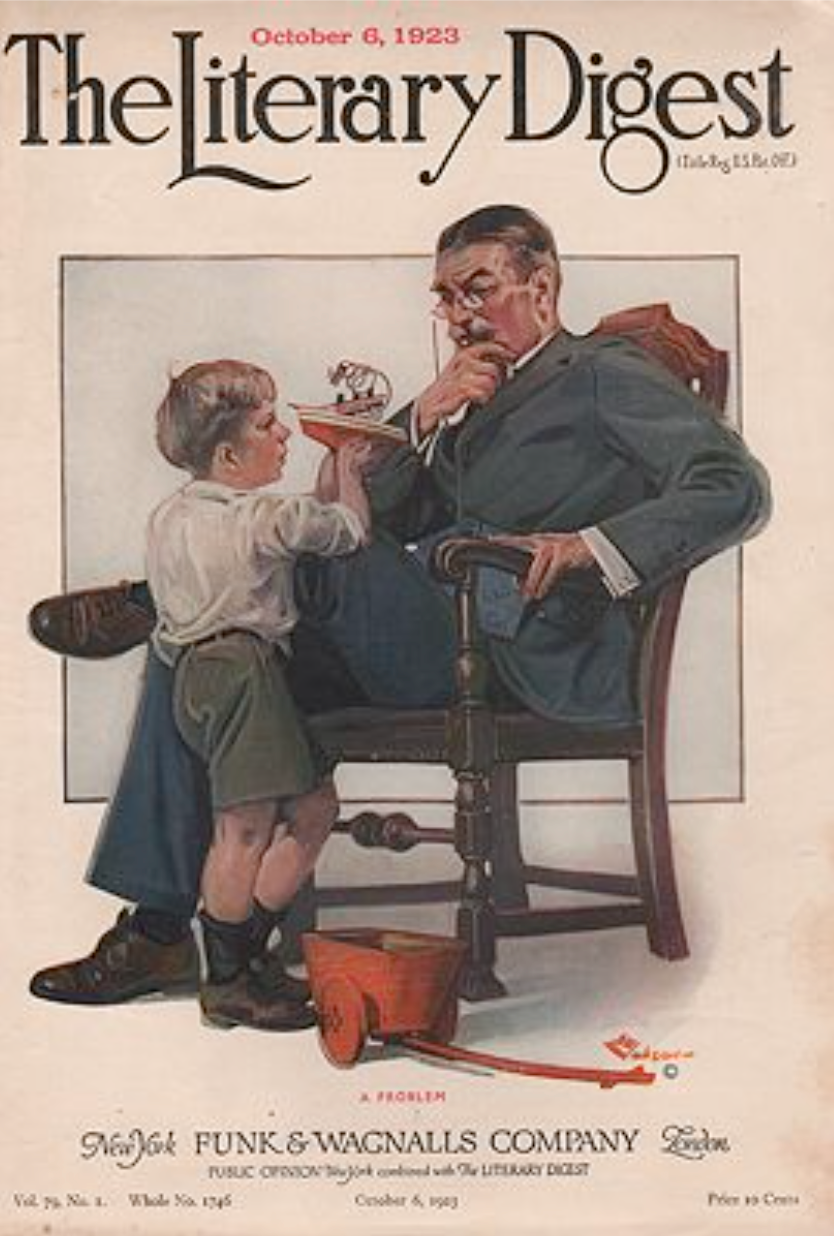
\includegraphics[scale=0.3]{LD.png}
%\end{center}
%\end{column}
%\end{columns}
%
%\end{frame}

%@@@@@@@@@@@@@@@@@@@@@@@@@@@@@@@@@@@@@@@@@@@@@@@@@
\begin{frame}
\frametitle{Bernoulli Random Variables}

\begin{itemize}
\item A \textbf{Bernoulli random variable} is used to model the outcome of an experiment that can be answered as a \textbf{boolean} -- typical answers could be:
\begin{itemize}
\item  Yes or No;
\item Success or Failure;
\item True or False;
\item $1$ or $0$;
\end{itemize}
\bigskip

\item Has a probability distribution with a single parameter: $\pi$, the probability of Yes/Success/True/1;
\bigskip

\item Let's take the outcomes to be 0 and 1.  Then we can write this as a function:
\begin{align*}
p(k = 1,\pi) &= \color{white}\pi\\
\color{white}p(k = 0,\pi) &\color{white}= 1 - \pi\\
\color{white}p(k,\pi) &\color{white}= \pi^k(1-\pi)^{1-k} \mbox{ for }k = 0\mbox{ or }k = 1.
\end{align*}

\end{itemize}

\end{frame}

%@@@@@@@@@@@@@@@@@@@@@@@@@@@@@@@@@@@@@@@@@@@@@@@@@
\begin{frame}
\frametitle{Bernoulli Random Variables}

\begin{itemize}
\item A \textbf{Bernoulli random variable} is used to model the outcome of an experiment that can be answered as a \textbf{boolean} -- typical answers could be:
\begin{itemize}
\item  Yes or No;
\item Success or Failure;
\item True or False;
\item $1$ or $0$;
\end{itemize}
\bigskip

\item Has a probability distribution with a single parameter: $\pi$, the probability of Yes/Success/True/1;
\bigskip

\item Let's take the outcomes to be 0 and 1.  Then we can write this as a function:
\begin{align*}
p(k = 1,\pi) &= \pi\\
p(k = 0,\pi) &= \color{white}1 - \pi\\
\color{white}p(k,\pi) &\color{white}= \pi^k(1-\pi)^{1-k} \mbox{ for }k = 0\mbox{ or }k = 1.
\end{align*}

\end{itemize}

\end{frame}

%@@@@@@@@@@@@@@@@@@@@@@@@@@@@@@@@@@@@@@@@@@@@@@@@@
\begin{frame}
\frametitle{Bernoulli Random Variables}

\begin{itemize}
\item A \textbf{Bernoulli random variable} is used to model the outcome of an experiment that can be answered as a \textbf{boolean} -- typical answers could be:
\begin{itemize}
\item  Yes or No;
\item Success or Failure;
\item True or False;
\item $1$ or $0$;
\end{itemize}
\bigskip

\item Has a probability distribution with a single parameter: $\pi$, the probability of Yes/Success/True/1;
\bigskip

\item Let's take the outcomes to be 0 and 1.  Then we can write this as a function:
\begin{align*}
p(k = 1,\pi) &= \pi\\
p(k = 0,\pi) &= 1 - \pi\\
p(k,\pi) &=\color{white} \pi^k(1-\pi)^{1-k} \mbox{ for }k = 0\mbox{ or }k = 1.
\end{align*}

\end{itemize}

\end{frame}

%@@@@@@@@@@@@@@@@@@@@@@@@@@@@@@@@@@@@@@@@@@@@@@@@@
\begin{frame}
\frametitle{Bernoulli Random Variables}

\begin{itemize}
\item A \textbf{Bernoulli random variable} is used to model the outcome of an experiment that can be answered as a \textbf{boolean} -- typical answers could be:
\begin{itemize}
\item  Yes or No;
\item Success or Failure;
\item True or False;
\item $1$ or $0$;
\end{itemize}
\bigskip

\item Has a probability distribution with a single parameter: $\pi$, the probability of Yes/Success/True/1;
\bigskip

\item Let's take the outcomes to be 0 and 1.  Then we can write this as a function:
\begin{align*}
p(k = 1,\pi) &= \pi\\
p(k = 0,\pi) &= 1 - \pi\\
\mbox{or: }p(k,\pi) &= \pi^k(1-\pi)^{1-k} \mbox{ for }k = 0\mbox{ or }k = 1.
\end{align*}

\end{itemize}

\end{frame}

%@@@@@@@@@@@@@@@@@@@@@@@@@@@@@@@@@@@@@@@@@@@@@@@@@
\begin{frame}
\frametitle{Binomial Random Variables}

\begin{itemize}
\item A \textbf{binomial random variable} is used to model the sum of $n$ Bernoulli experiments -- how many successes after $n$ tries?
\bigskip

\item Has a probability distribution with three parameters:
\begin{enumerate}
\item $n$, the number of tries;
\item $k$, the number of successes;
\item $\pi$, the probability of each success;
\end{enumerate}
\bigskip

\item If we had a single try we could have either $k = 1$ success or $k=0$ successes:
\begin{align*}
p(k = 1,n=1,\pi) & = \pi\\
p(k = 0,n=1,\pi) & = 1 - \pi\\
\mbox{or: }p(k,n=1,\pi) &= \pi^k(1-\pi)^{1-k}.
\end{align*}

\end{itemize}

\end{frame}

%@@@@@@@@@@@@@@@@@@@@@@@@@@@@@@@@@@@@@@@@@@@@@@@@@
\begin{frame}
\frametitle{Binomial Random Variables}

\begin{itemize}
\item A \textbf{binomial random variable} is used to model the sum of $n$ Bernoulli experiments -- how many successes after $n$ tries?
\bigskip

\item Has a probability distribution with three parameters:
\begin{enumerate}
\item $n$, the number of tries;
\item $k$, the number of successes;
\item $\pi$, the probability of each success;
\end{enumerate}
\bigskip

\item If we had two tries we could have $k=2,1$ or $0$ successes:
\begin{align*}
p(k = 2,n=2,\pi) & = \pi^2\\
p(k = 1,n=2,\pi) & = \pi(1-\pi) + (1-\pi)\pi\\
p(k = 0,n=2,\pi) & = (1 - \pi)^2\\
\mbox{or: }p(k,n=2,\pi) & \propto \pi^k(1-\pi)^{2-k}.
\end{align*}


\end{itemize}

\end{frame}

%@@@@@@@@@@@@@@@@@@@@@@@@@@@@@@@@@@@@@@@@@@@@@@@@@
\begin{frame}
\frametitle{Binomial Random Variables}

\begin{itemize}
\item A \textbf{binomial random variable} is used to model the sum of $n$ Bernoulli experiments -- how many successes after $n$ tries?
\bigskip

\item Has a probability distribution with three parameters:
\begin{enumerate}
\item $n$, the number of tries;
\item $k$, the number of successes;
\item $\pi$, the probability of each success;
\end{enumerate}
\bigskip

\item If we had three tries we could have $k=3,2,1$ or $0$ successes:
\begin{align*}
p(k,\pi) \propto \pi^k(1-\pi)^{3-k}.
\end{align*}

\end{itemize}

\end{frame}

%@@@@@@@@@@@@@@@@@@@@@@@@@@@@@@@@@@@@@@@@@@@@@@@@@
\begin{frame}
\frametitle{Binomial Random Variables}

\begin{itemize}
\item A \textbf{binomial random variable} is used to model the sum of $n$ Bernoulli experiments -- how many successes after $n$ tries?
\bigskip

\item Has a probability distribution with three parameters:
\begin{enumerate}
\item $n$, the number of tries;
\item $k$, the number of successes;
\item $\pi$, the probability of each success;
\end{enumerate}
\bigskip

\item If we had $n$ tries we could have $k=n,\hdots,3,2,1$ or $0$ successes:
\begin{align*}
p(k,\pi) \propto \pi^k(1-\pi)^{n-k}.
\end{align*}

\end{itemize}

\end{frame}

%@@@@@@@@@@@@@@@@@@@@@@@@@@@@@@@@@@@@@@@@@@@@@@@@@
\begin{frame}
\frametitle{Binomial Random Variables}

\begin{center}
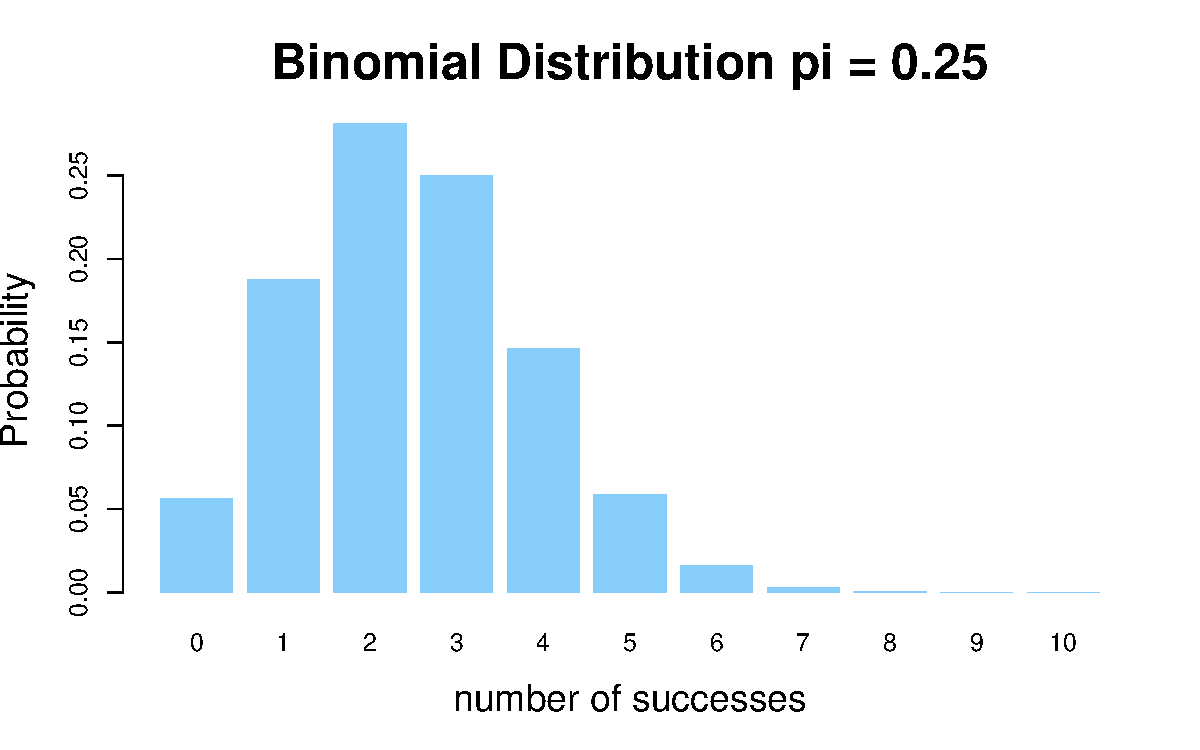
\includegraphics[scale=0.5]{binomial_25.pdf}
\end{center}

\end{frame}

%@@@@@@@@@@@@@@@@@@@@@@@@@@@@@@@@@@@@@@@@@@@@@@@@@
\begin{frame}
\frametitle{Binomial Random Variables}

\begin{center}
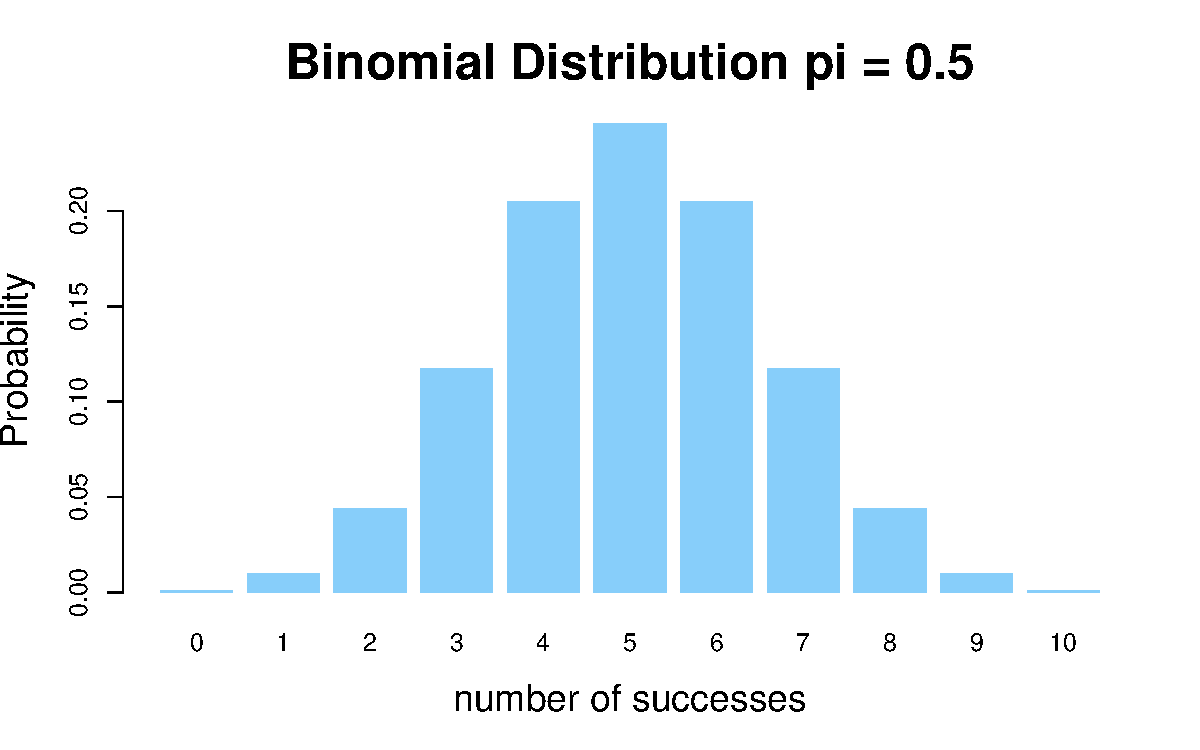
\includegraphics[scale=0.5]{binomial_5.pdf}
\end{center}

\end{frame}

%@@@@@@@@@@@@@@@@@@@@@@@@@@@@@@@@@@@@@@@@@@@@@@@@@
\begin{frame}
\frametitle{Binomial Random Variables}

\begin{center}
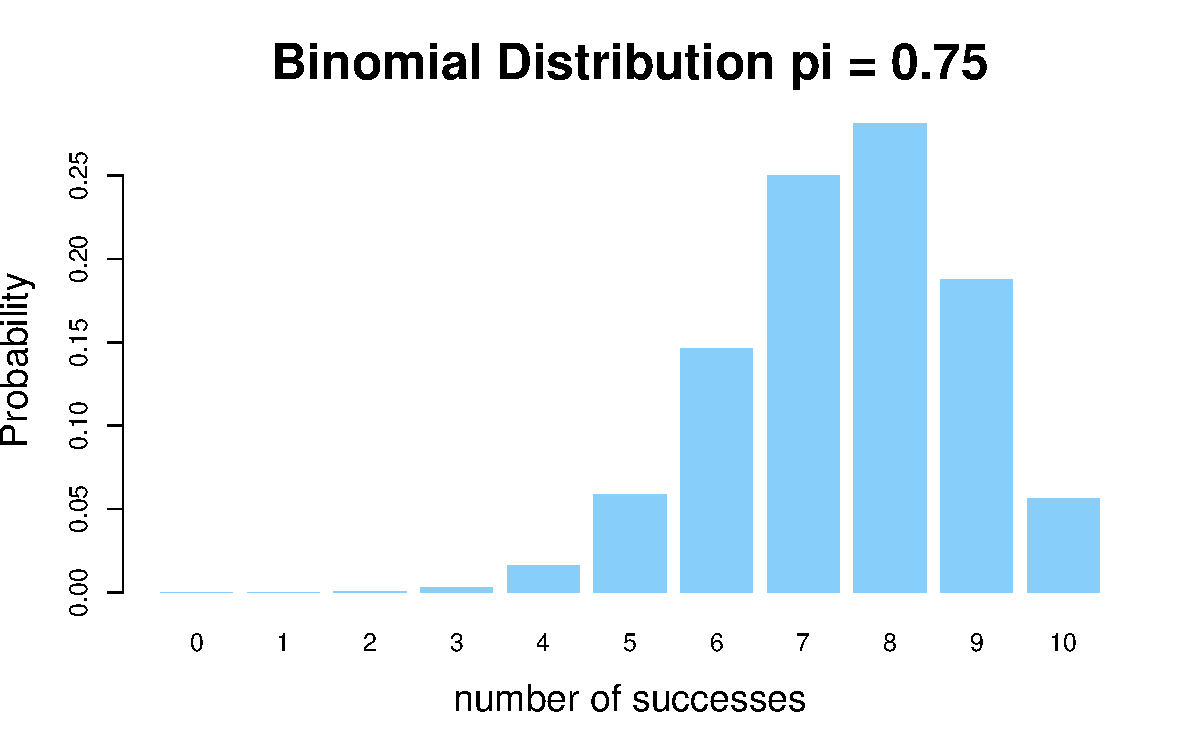
\includegraphics[scale=0.5]{binomial_75.pdf}
\end{center}

\end{frame}

%@@@@@@@@@@@@@@@@@@@@@@@@@@@@@@@@@@@@@@@@@@@@@@@@@
\begin{frame}
\frametitle{Normal Random Variables}

\begin{itemize}
\item \textbf{Normal random variables} can be used to model just about any interval or ratio data (so continuous data) -- why?
\bigskip

\item[]\color{white} \textbf{Reminder -- the central limit theorem}: As sample size gets bigger the sampling distribution of a sample statistic increasingly follows a normal distribution and the standard deviation of that normal distribution gets smaller;
\bigskip

\item[]\color{white} Has a probability distribution with two parameters: $\mu$, the mean and $\sigma$ the standard deviation:
\begin{align*}
\color{white}N(x,\mu,\sigma) = \frac{1}{\sqrt{2*3.1416*\sigma^2}}\exp\left\{-\frac{(x - \mu)^2}{2\sigma^2}\right\};
\end{align*}

\item[]\color{white} When $\mu = 0$ and $\sigma = 1$ we call it the \textbf{standard normal}:
\begin{align*}
\color{white}N(x,\mu=0,\sigma=1) = \frac{1}{\sqrt{2*3.1416}}\exp\left\{-\frac{x^2}{2}\right\}.
\end{align*}

\end{itemize}

\end{frame}

%@@@@@@@@@@@@@@@@@@@@@@@@@@@@@@@@@@@@@@@@@@@@@@@@@
\begin{frame}
\frametitle{Normal Random Variables}

\begin{itemize}
\item \textbf{Normal random variables} can be used to model just about any interval or ratio data (so continuous data) -- why?
\bigskip

\item \textbf{Reminder -- the central limit theorem}: As sample size gets bigger the sampling distribution of a sample statistic increasingly follows a normal distribution and the standard deviation of that normal distribution gets smaller;
\bigskip

\item[]\color{white} Has a probability distribution with two parameters: $\mu$, the mean and $\sigma$ the standard deviation:
\begin{align*}
\color{white}N(x,\mu,\sigma) = \frac{1}{\sqrt{2*3.1416*\sigma^2}}\exp\left\{-\frac{(x - \mu)^2}{2\sigma^2}\right\};
\end{align*}

\item[]\color{white} When $\mu = 0$ and $\sigma = 1$ we call it the \textbf{standard normal}:
\begin{align*}
\color{white}N(x,\mu=0,\sigma=1) = \frac{1}{\sqrt{2*3.1416}}\exp\left\{-\frac{x^2}{2}\right\}.
\end{align*}

\end{itemize}

\end{frame}

%@@@@@@@@@@@@@@@@@@@@@@@@@@@@@@@@@@@@@@@@@@@@@@@@@
\begin{frame}
\frametitle{Normal Random Variables}

\begin{itemize}
\item \textbf{Normal random variables} can be used to model just about any interval or ratio data (so continuous data) -- why?
\bigskip

\item \textbf{Reminder -- the central limit theorem}: As sample size gets bigger the sampling distribution of a sample statistic increasingly follows a normal distribution and the standard deviation of that normal distribution gets smaller;
\bigskip

\item Has a probability distribution with two parameters: $\mu$, the mean and $\sigma$ the standard deviation:
\begin{align*}
N(x,\mu,\sigma) = \frac{1}{\sqrt{2*3.1416*\sigma^2}}\exp\left\{-\frac{(x - \mu)^2}{2\sigma^2}\right\};
\end{align*}

\item[]\color{white} When $\mu = 0$ and $\sigma = 1$ we call it the \textbf{standard normal}:
\begin{align*}
\color{white}N(x,\mu=0,\sigma=1) = \frac{1}{\sqrt{2*3.1416}}\exp\left\{-\frac{x^2}{2}\right\}.
\end{align*}

\end{itemize}

\end{frame}

%@@@@@@@@@@@@@@@@@@@@@@@@@@@@@@@@@@@@@@@@@@@@@@@@@
\begin{frame}
\frametitle{Normal Random Variables}

\begin{itemize}
\item \textbf{Normal random variables} can be used to model just about any interval or ratio data (so continuous data) -- why?
\bigskip

\item \textbf{Reminder -- the central limit theorem}: As sample size gets bigger the sampling distribution of a sample statistic increasingly follows a normal distribution and the standard deviation of that normal distribution gets smaller;
\bigskip

\item Has a probability distribution with two parameters: $\mu$, the mean and $\sigma$ the standard deviation:
\begin{align*}
N(x,\mu,\sigma) = \frac{1}{\sqrt{2*3.1416*\sigma^2}}\exp\left\{-\frac{(x - \mu)^2}{2\sigma^2}\right\};
\end{align*}

\item When $\mu = 0$ and $\sigma = 1$ we call it the \textbf{standard normal}:
\begin{align*}
N(x,\mu=0,\sigma=1) = \frac{1}{\sqrt{2*3.1416}}\exp\left\{-\frac{x^2}{2}\right\}.
\end{align*}

\end{itemize}

\end{frame}

%@@@@@@@@@@@@@@@@@@@@@@@@@@@@@@@@@@@@@@@@@@@@@@@@@
\begin{frame}
\frametitle{Normal -- what happens as mean changes?}

\begin{center}
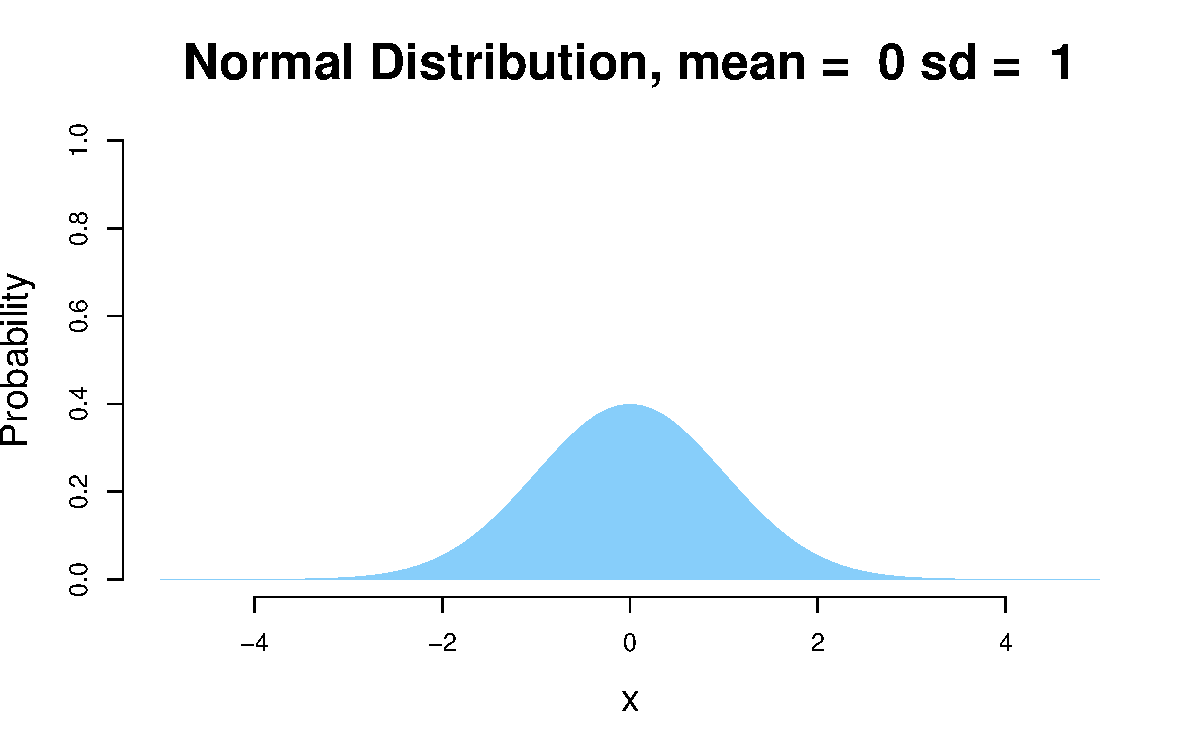
\includegraphics[scale=0.5]{Normal_0_1.pdf}
\end{center}

\end{frame}

%@@@@@@@@@@@@@@@@@@@@@@@@@@@@@@@@@@@@@@@@@@@@@@@@@
\begin{frame}
\frametitle{Normal -- what happens as mean changes?}

\begin{center}
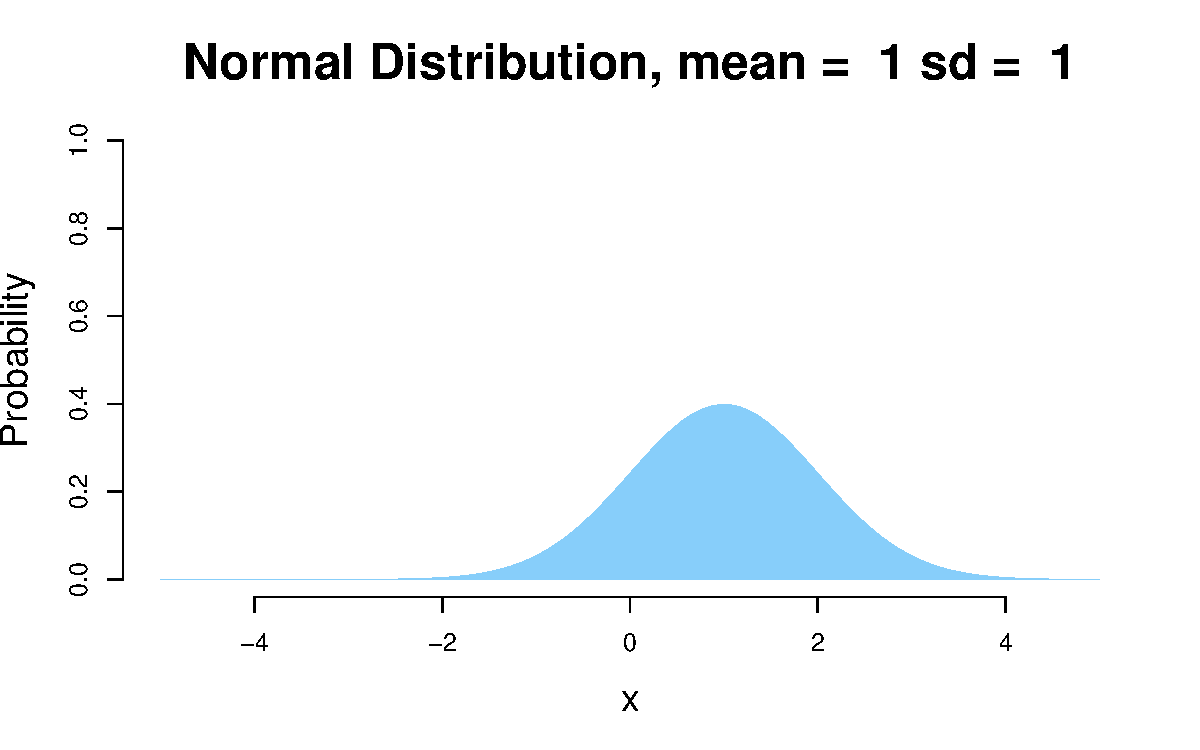
\includegraphics[scale=0.5]{Normal_1_1.pdf}
\end{center}

\end{frame}

%@@@@@@@@@@@@@@@@@@@@@@@@@@@@@@@@@@@@@@@@@@@@@@@@@
\begin{frame}
\frametitle{Normal -- what happens as mean changes?}

\begin{center}
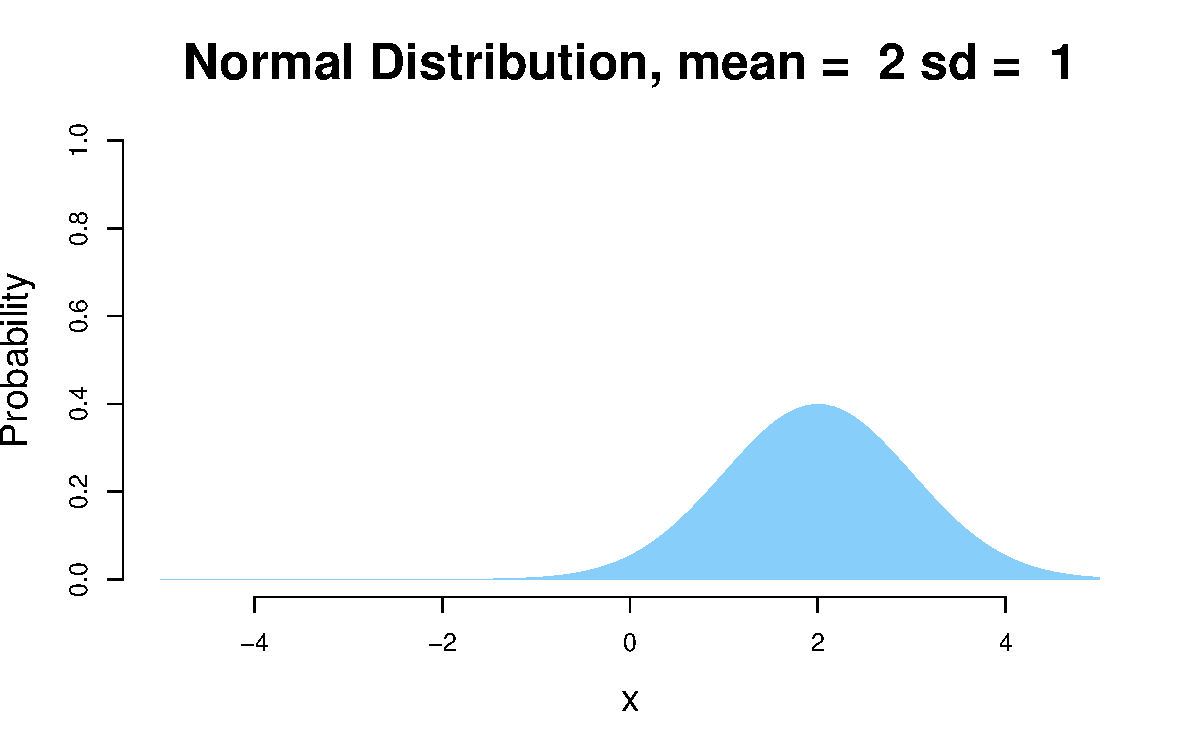
\includegraphics[scale=0.5]{Normal_2_1.pdf}
\end{center}

\end{frame}

%@@@@@@@@@@@@@@@@@@@@@@@@@@@@@@@@@@@@@@@@@@@@@@@@@
\begin{frame}
\frametitle{Normal -- what happens as standard deviation changes?}

\begin{center}
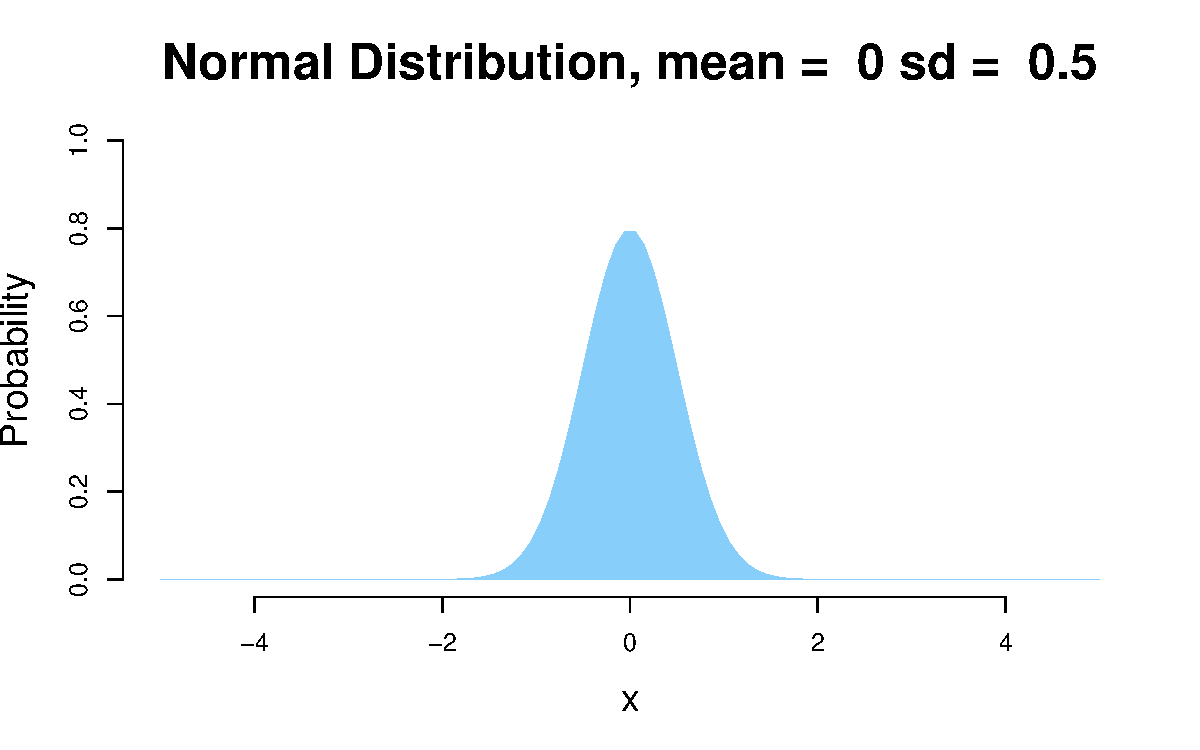
\includegraphics[scale=0.5]{Normal_0_0.5.pdf}
\end{center}

\end{frame}

%@@@@@@@@@@@@@@@@@@@@@@@@@@@@@@@@@@@@@@@@@@@@@@@@@
\begin{frame}
\frametitle{Normal -- what happens as standard deviation changes?}

\begin{center}
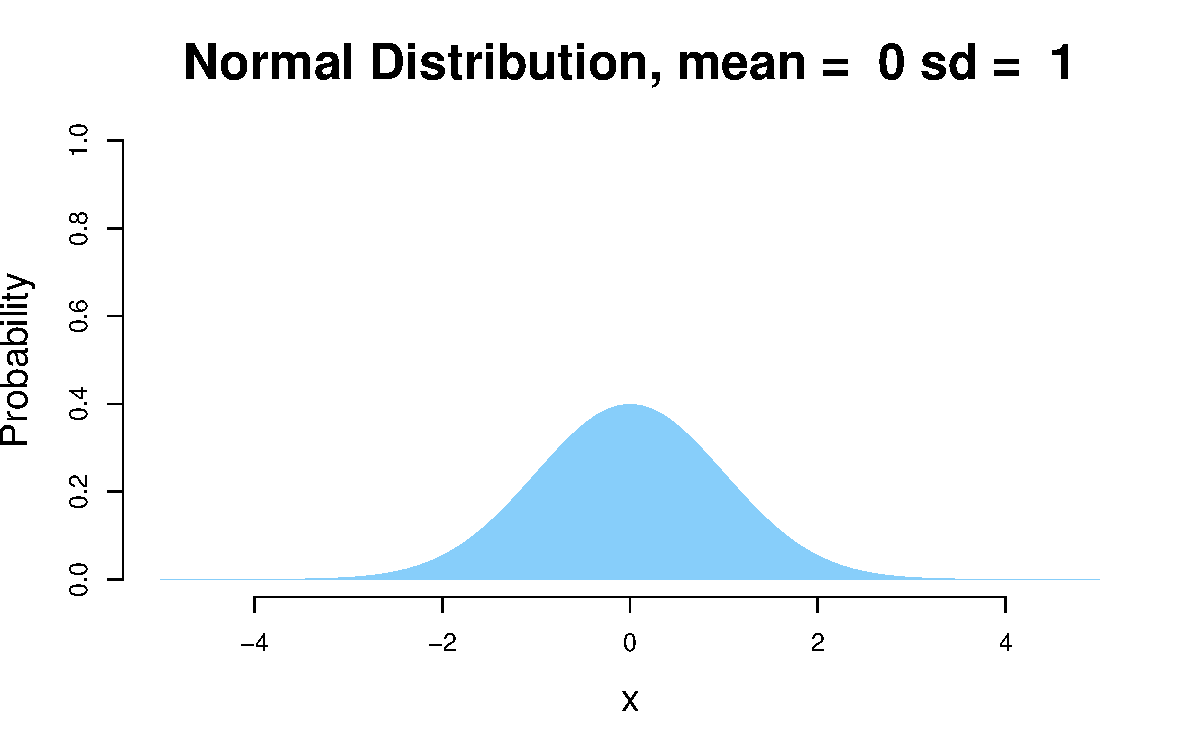
\includegraphics[scale=0.5]{Normal_0_1.pdf}
\end{center}

\end{frame}

%@@@@@@@@@@@@@@@@@@@@@@@@@@@@@@@@@@@@@@@@@@@@@@@@@
\begin{frame}
\frametitle{Normal -- what happens as standard deviation changes?}

\begin{center}
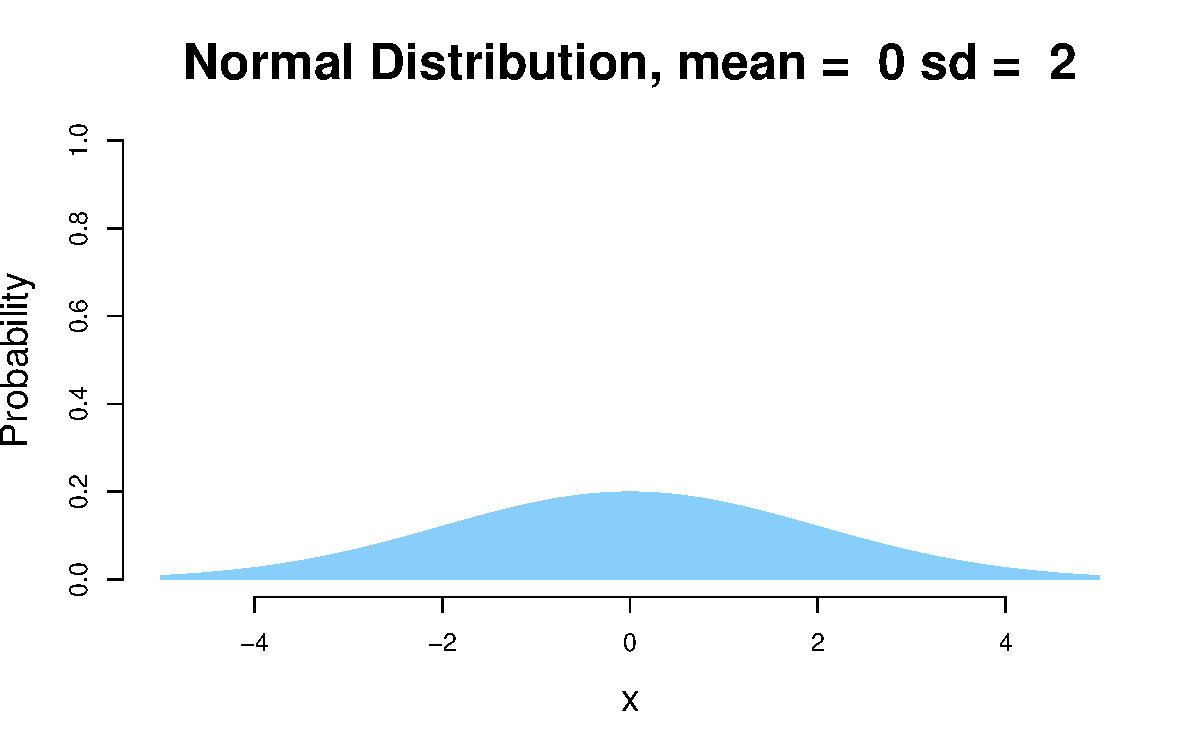
\includegraphics[scale=0.5]{Normal_0_2.pdf}
\end{center}

\end{frame}

%@@@@@@@@@@@@@@@@@@@@@@@@@@@@@@@@@@@@@@@@@@@@@@@@@
\begin{frame}
\frametitle{Motivation -- reasoning about voters...}

\begin{columns}
\begin{column}{0.5\textwidth}

\begin{itemize}
\item Cavalier Johnson: a political candidate running a campaign for Mayor of Milwaukee;
\bigskip

\item Johnson's campaign claims that he will win the election -- in this case that means getting more than 50\% of votes from Milwaukee voters;
\bigskip

\item How to assess the Johnson campaign claim?  Conduct an experiment:
\begin{itemize}
\item \textbf{Sample} $n$ voters from Milwaukee;
\item Record the number of voters who will vote for Johnson.
\end{itemize}

\end{itemize}

\end{column}
\begin{column}{0.5\textwidth}
\begin{center}
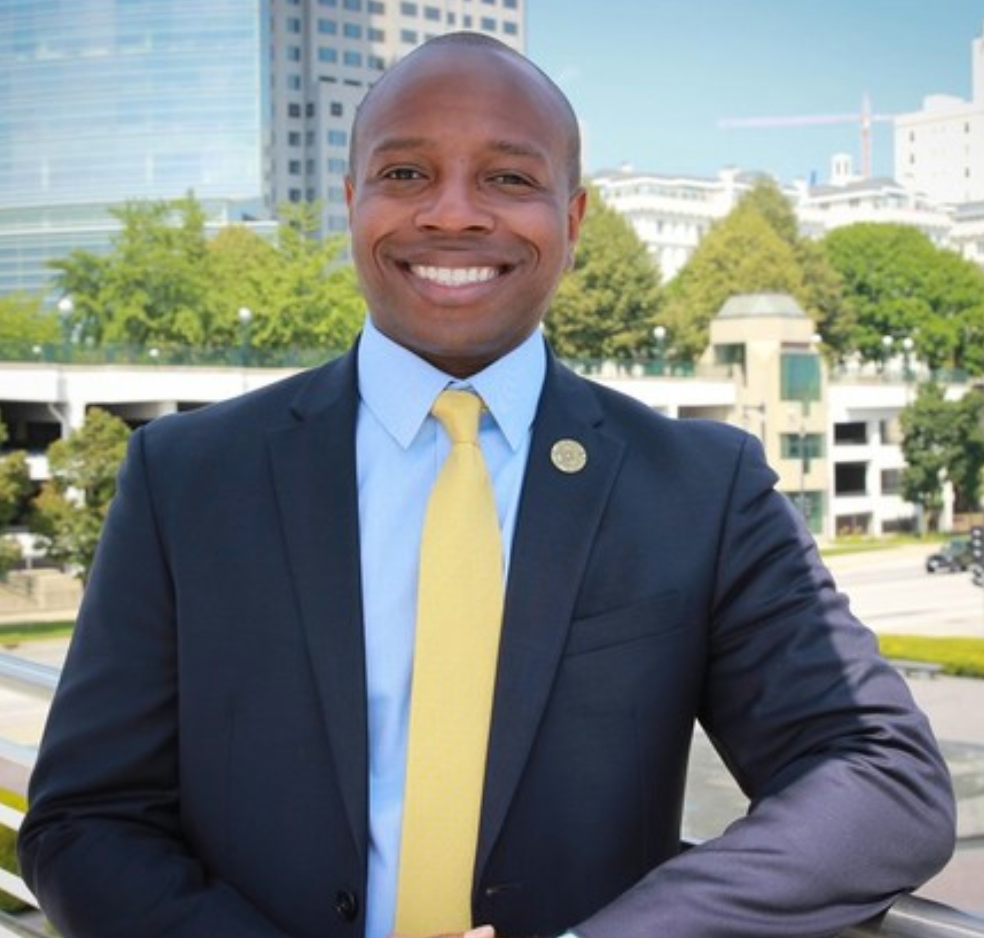
\includegraphics[scale=0.4]{Johnson.png}
\end{center}
\end{column}
\end{columns}

\end{frame}

%@@@@@@@@@@@@@@@@@@@@@@@@@@@@@@@@@@@@@@@@@@@@@@@@@
\begin{frame}


\begin{center}
\huge If we see that $k$ out of $n$ voters say they will vote for Johnson, what is the probability his campaign's claim is correct?
\end{center}

\end{frame}

%@@@@@@@@@@@@@@@@@@@@@@@@@@@@@@@@@@@@@@@@@@@@@@@@@
\begin{frame}

\begin{center}
\Huge\textbf{Why should we care?}\\
\bigskip
\bigskip
\large Probability is used for all hypothesis testing and statistical modeling.\\
\end{center}

\end{frame}



\end{document}






